\documentclass[preprint,authoryear,12pt]{elsarticle}

%% Use the option review to obtain double line spacing
%% \documentclass[authoryear,preprint,review,12pt]{elsarticle}

%% Use the options 1p,twocolumn; 3p; 3p,twocolumn; 5p; or 5p,twocolumn
%% for a journal layout:
%% \documentclass[final,authoryear,1p,times]{elsarticle}
%% \documentclass[final,authoryear,1p,times,twocolumn]{elsarticle}
%% \documentclass[final,authoryear,3p,times]{elsarticle}
%% \documentclass[final,authoryear,3p,times,twocolumn]{elsarticle}
%% \documentclass[final,authoryear,5p,times]{elsarticle}
%% \documentclass[final,authoryear,5p,times,twocolumn]{elsarticle}

\usepackage{graphicx}
\usepackage[cmex10]{amsmath}
\usepackage{array}
\usepackage{url}

\usepackage[utf8]{inputenc}
\usepackage{amsmath, amsthm, amssymb, bm}
\usepackage{verbatim}
\usepackage{graphicx}%\graphicspath{{figures/}}
\usepackage{multicol}
\usepackage{multirow}
\usepackage{tabularx}
%\usepackage[usenames]{color}
\usepackage{mathrsfs}
\usepackage[colorlinks,citecolor=blue,urlcolor=blue,linkcolor=blue]{hyperref}
\usepackage{hypernat}
\usepackage{datetime}
\usepackage{textcomp}
\usepackage{include/picins}
\usepackage{tikz}
\usetikzlibrary{shapes.geometric,arrows,chains,matrix,positioning,scopes,calc}
\tikzstyle{mybox} = [draw=white, rectangle]
\usepackage{booktabs}

\newcommand{\interrobang}{{\fontfamily{txr}\selectfont \textinterrobang}}

\theoremstyle{plain}

\def\ie{i.e.\ }
\def\eg{e.g.\ }
\def\indicator{\mathbb{I}}
\def\mean#1{\mathbb{E}[#1]}
\def\bigmean#1{\mathbb{E}\bigl[#1\bigr]}
\def\Bigmean#1{\mathbb{E}\Bigl[#1\Bigr]}
\def\cyl{\mathcal{Z}}
\def\eqae{=_{\mbox{\tiny a.e.}}}
\def\wrt{w.r.t.\ }
\def\ae{a.e.\ }
\def\equas{=_{\mbox{\tiny a.s.}}}
\def\equae{=_{\mbox{\tiny a.e.}}}
\def\iid{i.i.d.\ }
\def\Iid{I.i.d.\ }
%\def\inclusion{\jmath}
\def\inclusion{\mathcal{J}}
\def\inclusionX{\inclusion_{\xspace}}
\def\wstar{weak$^{\ast}$ }
% Symmetric difference
\def\symmdiff{\!\vartriangle\!}


% Indices

\def\indI{\mbox{\tiny I}}
\def\indJ{\mbox{\tiny J}}
\def\indK{\mbox{\tiny K}}
\def\indJI{\mbox{\tiny J$\setminus$I}}
\def\indE{\mbox{\tiny E}}
\def\indF{\mbox{\tiny F}}
\def\indD{\mbox{\tiny D}}
\def\indi{\mbox{\tiny{\{i\}}}}
\def\ind#1{\mbox{\tiny #1}}
\def\power{\mathcal{F}}
\def\powerD{\power(D)}
\def\powerE{\power(E)}
\def\powerL{\power(L)}
\def\parts{\mathcal{H}}
\def\partsQ{\parts(\mathcal{Q})}
\def\partsn{\parts[n]}
\def\partsN{\parts_{\infty}(\mathbb{N})}

% Spaces

\def\abstspace{\Omega}
\def\xspace{\mathcal{X}}
\def\yspace{\mathcal{Y}}
\def\tspace{\mathcal{T}}
\def\xspaceI{\xspace_{\indI}}
\def\xspaceJ{\xspace_{\indJ}}
\def\xspaceD{\xspace_{\indD}}
\def\xspaceE{\xspace_{\indE}}
\def\tspaceI{\tspace_{\indI}}
\def\tspaceJ{\tspace_{\indJ}}
\def\tspaceD{\tspace_{\indD}}
\def\tspaceE{\tspace_{\indE}}
\def\txspace{\tilde{\xspace}}
\def\yspaceI{\yspace_{\indI}}
\def\yspaceJ{\yspace_{\indJ}}
\def\yspaceD{\yspace_{\indD}}
\def\yspaceE{\yspace_{\indE}}
\def\txspace{\tilde{\xspace}}
\def\ttspace{\tilde{\tspace}}
\def\xI{x_{\indI}}
\def\xJ{x_{\indJ}}
\def\xD{x_{\indD}}
\def\xE{x_{\indE}}
\def\tImage{\Gamma}
\def\simp{\triangle}
\def\simpI{\simp_{\indI}}
\def\simpJ{\simp_{\indJ}}

\def\AI{A_{\indI}}
\def\AJ{A_{\indJ}}
\def\AD{A_{\indD}}
\def\AE{A_{\indE}}


%Space of Prob Measures
\def\pMeas{M}
%Space of Contents
\def\fMeas{N}
%Space of cont fcts
\def\cfspace{C}
%Hilbert space
\def\hilbert{\mathcal{L}^2}


\def\borelV{\borel_{V}}

% Set systems

\def\borel{\mathcal{B}}
\def\top{\mbox{Top}}

\def\borelI{\borel_{\indI}}
\def\borelJ{\borel_{\indJ}}
\def\borelD{\borel_{\indD}}
\def\borelE{\borel_{\indE}}
\def\tborel{\tilde{\borel}}
\def\abstfield{\mathcal{A}}
\def\field{\mathcal{C}}
\def\fieldI{\field_{\indI}}
\def\fieldJ{\field_{\indJ}}
\def\fieldK{\field_{\indK}}
\def\fieldD{\field_{\indD}}
\def\fieldE{\field_{\indE}}
\def\tfield{\tilde{\mathcal{C}}}
\def\Sfield{\mathcal{S}}
\def\SfieldI{\mathcal{S}_{\indI}}
\def\SfieldJ{\mathcal{S}_{\indJ}}
\def\SfieldD{\mathcal{S}_{\indD}}
\def\tSfield{\tilde{\mathcal{S}}}
\def\borelx{\borel_x}
\def\tborelx{\tborel_x}
\def\borelgamma{\tborel_{\tImage}}
%\def\borelth{\borel_{\theta}}
\def\borely{\borel_{y}}
%\def\borelT{\borel_t}
\def\borelT{\borel_{\tspace}}
\def\borelS{\borel_s}
\def\topI{\top_{\indI}}
\def\topJ{\top_{\indJ}}
\def\topD{\top_{\indD}}
\def\topE{\top_{\indE}}
\def\topV{\top_V}
\def\topws{\top_{\text{ws}}}
\def\topcc{\top_{\text{c}}}
\def\borelXI{\borel(\xspaceI)}
\def\borelXD{\borel(\xspaceD)}
\def\tborelX{\borel(\txspace)}
\def\borelTI{\borel(\tspaceI)}
\def\borelTD{\borel(\tspaceD)}
\def\tborelT{\borel(\ttspace)}


% Maps

\def\XI{X_{\indI}}
\def\Xi{X_{\ind{i}}}
\def\Xj{X_{\ind{j}}}
\def\ThetaI{\Theta_{\indI}}
\def\XJ{X_{\indJ}}
\def\ThetaJ{\Theta_{\indJ}}
\def\XD{X_{\indD}}
\def\ThetaD{\Theta_{\indD}}
\def\XE{X_{\indE}}
\def\ThetaE{\Theta_{\indE}}
\def\tX{\tilde{X}}
\def\tTheta{\tilde{\Theta}}

\def\SI{S_{\indI}}
\def\TI{T_{\indI}}

\def\rest{\phi}
\def\restD{\rest_{\indD}}
\def\restI{\rest_{\indI}}
\def\restJ{\rest_{\indJ}}
\def\restDI{\rest^{\indD}_{\indI}}
\def\inclusionD{\inclusion_{\indD}}
\def\inclusionE{\inclusion_{\indE}}
\def\projector{\mbox{pr}}
\def\projectorD{\projector_{\indD}}
\def\projectorI{\projector_{\indI}}
\def\projectorJI{\pi_{\indJ\indI}}
\def\indicator{\mathbb{I}}

% Projective systems

\def\po{\preceq}
\def\famD#1{{\lbrace #1 \rbrace}_{\indD}}
\def\famE#1{{\lbrace #1 \rbrace}_{\ind{I$\in$}\indE}}
\def\fJI{f_{\indJ\indI}}
\def\fKI{f_{\indK\indI}}
\def\fKJ{f_{\indK\indJ}}
\def\fII{f_{\indI\indI}}
\def\fI{f_{\indI}}
\def\fJ{f_{\indJ}}
\def\fK{f_{\indK}}
\def\fD{f_{\indD}}
\def\fDI{f^{\indD}_{\indI}}
\def\fDK{f^{\indD}_{\indK}}
\def\gJI{g_{\indJ\indI}}
\def\gI{g_{\indI}}
\def\gJ{g_{\indJ}}
\def\gD{g_{\indD}}
\def\hJI{h_{\indJ\indI}}
\def\hI{h_{\indI}}
\def\hJ{h_{\indJ}}
\def\hE{h_{\indE}}
\def\plim{\varprojlim}

% Measure and Conditionals

\def\abstmeasure{\mathbb{P}}
\def\P{P}
\def\PI{P_{\indI}}
\def\PJ{P_{\indJ}}
\def\PD{P_{\indD}}
\def\PE{P_{\indE}}
\def\PX{P_{\mbox{X}}}
\def\PTh{P_{\mbox{\Theta}}}
\def\PXI{P_{\XI}}
\def\PThI{P_{\mbox{\Theta}}}
\def\PXJ{P_{\mbox{X}}}
\def\PThJ{P_{\mbox{\Theta}}}
\def\PXD{P_{\mbox{X}}}
\def\PThD{P_{\mbox{\Theta}}}
\def\PXE{P_{\mbox{X}}}
\def\PThE{P_{\mbox{\Theta}}}
\def\tP{\tilde{P}}
\def\tPX{\tilde{P}_X}
\def\tPTh{\tilde{P}_{\Theta}}







\def\SI{S_{\indI}}
\def\SJ{S_{\indJ}}

\def\tk{\tilde{k}}
\def\kI{k_{\indI}}

\def\postkernel{k}
\def\indctr{\mathbbm{1}}
\def\sp#1{\left<#1\right>}


%Mallows
\def\Sr{\mathbb{S}_r}
\def\Sinf{\mathbb{S}_{\infty}}
\def\Sbar{\bar{\mathbb{S}}}
\def\DP#1{\mbox{DP}\left( #1 \right)}
\def\GP#1{\mbox{GP}\left( #1 \right)}
\def\x{\mathbf{x}}
\def\y{\mathbf{y}}



\def\tyspace{\tilde{\yspace}}
\def\tF{\tilde{F}}
\def\tT{\tilde{T}}
\def\tmodel{\tilde{\model}}
\def\tnu{\tilde{\nu}}


\def\PTheta{P^{\theta}}
\def\FTheta{F^{\theta}}
\def\TTheta{T^{\theta}}
\def\borelY{\borel_{\yspace}}

\def\PX{P^{x}}
\def\PXI{\PX_{\indI}}
\def\PXJ{\PX_{\indJ}}
\def\PXD{\PX_{\indD}}
\def\PThetaI{\PTheta_{\indI}}
\def\PThetaD{\PTheta_{\indD}}
\def\YI{Y_{\indI}}
\def\YJ{Y_{\indJ}}
\def\YD{Y_{\indD}}
\def\Tn{T^{(n)}}
\def\indexspace{\mathcal{W}}
\def\tyspace{\tilde{\yspace}}
\def\tY{\tilde{Y}}
\def\inclusionT{\inclusion_{\tspace}}
\def\tPTheta{\tilde{P}^{\theta}}
\def\tTn{\tilde{T}^{(n)}}
\def\inclusionY{\inclusion_{\yspace}}

\def\tyspace{\tilde{\yspace}}
\def\tF{\tilde{F}}
\def\tT{\tilde{T}}
\def\tmodel{\tilde{\model}}
\def\tnu{\tilde{\nu}}
\def\tOmega{\tilde{\abstspace}}
\def\tabstmeasure{\tilde{\abstmeasure}}
\def\model{\mathcal{P}}

\def\tf{\tilde{f}}
\def\tx{\tilde{x}}
\def\Dom{\mbox{Dom}}
\def\ty{\tilde{y}}

%Extra stuff - to be integrated in the future

\newcommand{\eqd}{\overset{\,_{\!d}}{=}}
\newcommand{\defn}[1]{\emph{#1}}

\newcommand{\Law}{\mathcal{L}}

\def\given{\,|\,}

\newcommand{\NonNegInts}{\mathbb{Z}_+}
\newcommand{\Nats}{\mathbb{N}}
\newcommand{\Rationals}{\mathbb{Q}}
\newcommand{\Reals}{\mathbb{R}}

\newcommand{\as}{\textrm{a.s.}}

\def\[#1\]{\begin{align}#1\end{align}}
\newcommand{\defas}{:=}

\newcommand{\Normal}{\mathcal{N}}
\newcommand{\dist}{\ \sim\ }

\newcommand{\kernel}{\kappa}
\newcommand{\kernelmatrix}{K}
\newcommand{\scalefactor}{s}
\newcommand{\lengthscale}{\ell}
\newcommand{\targets}{T}
\newcommand{\noise}{\sigma_\targets}
\newcommand{\pseudopoints}{\eta}
\newcommand{\inputpoints}{\xi}
\newcommand{\covhyppar}{\psi}
\newcommand{\logistic}{\phi}

\newcommand{\CompOrder}{\mathcal{O}}

\newtheorem{thm}{Theorem}%[section]
\newtheorem{lem}[thm]{Lemma}
\newtheorem{prop}[thm]{Proposition}
\newtheorem{cor}[thm]{Corollary}

\theoremstyle{definition}
\newtheorem{definition}[thm]{Definition}%[section]
\newtheorem{conj}{Conjecture}[section]
\newtheorem{exmp}{Example}[section]
\newtheorem{rem}[thm]{Remark}

\theoremstyle{remark}
%\newtheorem{rem}{Remark}
\newtheorem{note}{Note}
\newtheorem{case}{Case}

\def\Uniform{\mbox{\rm Uniform}}
\def\Bernoulli{\mbox{\rm Bernoulli}}
\def\ie{i.e.\ }
\def\eg{e.g.\ }
\def\etc{etc.\ }
\def\iid{i.i.d.\ }
\def\simiid{\sim_{\mbox{\tiny iid}}}
\def\eqdist{\stackrel{\mbox{\tiny d}}{=}}
\def\GP{\mathcal{GP}}
\def\Transpose{^\textrm{T}}

%%%%%%%%%%%%%%%%%%%%%%%%%%%%%%%%%%%%%%%%%%%%%%%%%%%%%%%%%%
%%%% EDITING HELPER FUNCTIONS  %%%%%%%%%%%%%%%%%%%%%%%%%%%
%%%%%%%%%%%%%%%%%%%%%%%%%%%%%%%%%%%%%%%%%%%%%%%%%%%%%%%%%%

%% NA: needs attention (rough writing whose correctness needs to be verified)
%% TBD: instructions for how to fix a gap ("Describe the propagation by ...")
%% PROBLEM: bug or missing crucial bit 

%% use \fXXX versions of these macros to put additional explanation into a footnote.  
%% The idea is that we don't want to interrupt the flow of the paper or make it 
%% impossible to read because there are a bunch of comments.

%% NA's (and TBDs, those less crucially) should be written so 
%% that they flow with the text.

\definecolor{WowColor}{rgb}{.75,0,.75}
\definecolor{SubtleColor}{rgb}{0,0,.50}

% inline
\newcommand{\NA}[1]{\textcolor{SubtleColor}{ {\tiny \bf ($\star$)} #1}}
\newcommand{\LATER}[1]{\textcolor{SubtleColor}{ {\tiny \bf ($\dagger$)} #1}}
\newcommand{\TBD}[1]{\textcolor{SubtleColor}{ {\tiny \bf (!)} #1}}
\newcommand{\PROBLEM}[1]{\textcolor{WowColor}{ {\bf (!!)} {\bf #1}}}

% as margin notes

\newcounter{margincounter}
\newcommand{\displaycounter}{{\arabic{margincounter}}}
\newcommand{\incdisplaycounter}{{\stepcounter{margincounter}\arabic{margincounter}}}

\newcommand{\fTBD}[1]{\textcolor{SubtleColor}{$\,^{(\incdisplaycounter)}$}\marginpar{\tiny\textcolor{SubtleColor}{ {\tiny $(\displaycounter)$} #1}}}

\newcommand{\fPROBLEM}[1]{\textcolor{WowColor}{$\,^{((\incdisplaycounter))}$}\marginpar{\tiny\textcolor{WowColor}{ {\bf $\mathbf{((\displaycounter))}$} {\bf #1}}}}

\newcommand{\fLATER}[1]{\textcolor{SubtleColor}{$\,^{(\incdisplaycounter\dagger)}$}\marginpar{\tiny\textcolor{SubtleColor}{ {\tiny $(\displaycounter\dagger)$} #1}}}


%% For submission, make all render blank.
%\renewcommand{\LATER}[1]{}
%\renewcommand{\fLATER}[1]{}
%\renewcommand{\TBD}[1]{}
%\renewcommand{\fTBD}[1]{}
%\renewcommand{\PROBLEM}[1]{}
%\renewcommand{\fPROBLEM}[1]{}  
%\renewcommand{\NA}[1]{#1}  %% Note, NA's pass through!

\journal{International Journal of Forecasting}

\begin{document}

\begin{frontmatter}

%% Title, authors and addresses

%% use the tnoteref command within \title for footnotes;
%% use the tnotetext command for the associated footnote;
%% use the fnref command within \author or \address for footnotes;
%% use the fntext command for the associated footnote;
%% use the corref command within \author for corresponding author footnotes;
%% use the cortext command for the associated footnote;
%% use the ead command for the email address,
%% and the form \ead[url] for the home page:
%%
\title{GEFCom2012 Load Forecasting \\ Gradient boosting machines and Gaussian processes}
%% \tnotetext[label1]{}
\author{James~Robert~Lloyd}
\ead{jrl44@cam.ac.uk}
%% \ead[url]{home page}
%% \fntext[label2]{}
%% \cortext[cor1]{}
\address{Department of Engineering, University of Cambridge}
%% \fntext[label3]{}

%% use optional labels to link authors explicitly to addresses:
%% \author[label1,label2]{<author name>}
%% \address[label1]{<address>}
%% \address[label2]{<address>}

\author{}

\address{}

\begin{abstract}
This report discusses methods for forecasting hourly loads of a US utility as part of the load forecasting track of the Global Energy Forecasting Competition 2012 hosted by Kaggle.
The methods described (gradient boosting machines and Gaussian processes) are generic machine learning / regression algorithms and few domain specific adjustments were made.
Despite this, the algorithms were able to produce highly competitive predictions and hopefully they can inspire more refined techniques to compete with state-of-the-art load forecasting methodologies.
\end{abstract}

\begin{keyword}
Utility forecasting \sep Gradient boosting machines \sep Gaussian processes
\end{keyword}

\end{frontmatter}

\section{Inroduction}

This report details the methods I used when competing in the load forecasting track of GEFCom2012\footnotemark.
\footnotetext{\url{http://www.gefcom.org/}}
It is split into sections describing each technique used for forecasting temperatures and loads.
Within each section I have motivated the particular choice of algorithm, discussed how it was used and described how to replicate the results using the spreadsheets and scripts accompanying this report\footnotemark.

\footnotetext{Available in the \texttt{clean\_nov} directory of the repository at \url{https://bitbucket.org/jamesrobertlloyd/gef_load}}

I approached the competition in the spirit of a data mining competition.
Consequently, some of the choices detailed below were based on intuition rather than objective analysis.
This was done purely to save time and focus on the aspects of the data most likely to give the largest increases in performance.
In general, many of the choices based on intuition could have been replaced by appropriate searches and cross validation; where more complex techniques would be required I have briefly described how one could perform a more objective analysis.

% You must have at least 2 lines in the paragraph with the drop letter
% (should never be an issue)

\section{Data cleaning}

Seemed ok - let algorithms look through noise.

\section{Weekends, holidays and other non-stationary phenomena}

Ignored

\section{Temperature forecasting}

\subsection{Initial analysis and remarks}

The error metric used in GEFCom2012 was heavily weighted towards load predictions at times at which temperatures were unknown (\ie the load forecast rather than backcast).
Consequently, good temperature predictions seemed crucial for overall success.
When optimising parameters of the temperature prediction methodology, my optimisation criterion was the public test score (as evaluated by Kaggle) of derived load prediction methods.

\begin{figure}[ht]
  \begin{center}
    \begin{tikzpicture}
  \begin{scope}[xshift=0cm]
    \node [mybox] (box){
      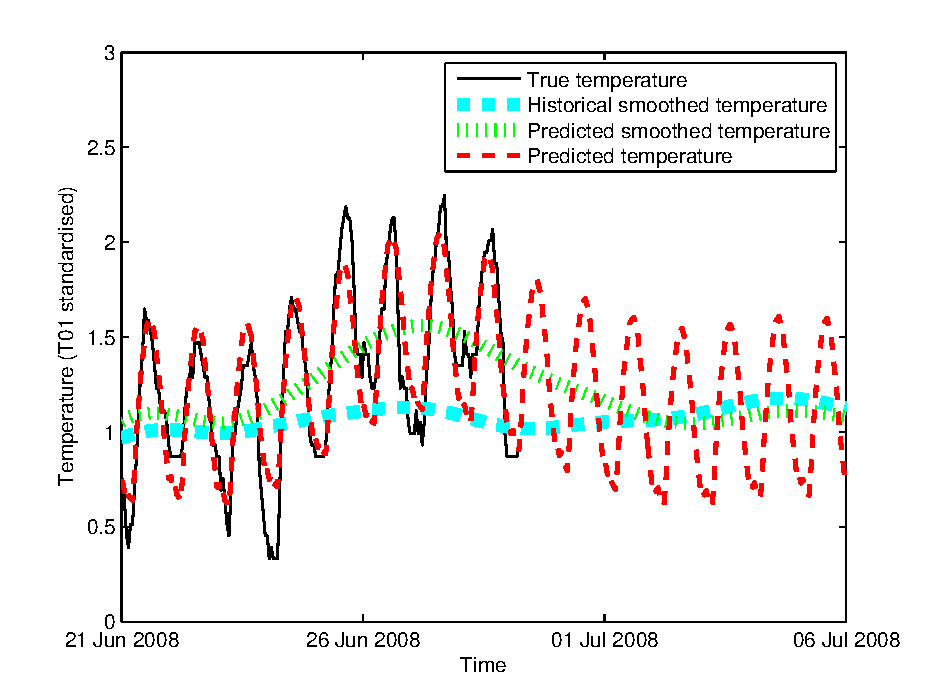
\includegraphics[width=0.7\textwidth]{../include/temp_pred.pdf}
    };
  \end{scope}
\end{tikzpicture}

  \end{center}
  \caption{Raw data at temperature station 1 (after removing mean and scaling to have unit standard deviation) (black). Historic average of smoothed temperatures (blue). Current and predicted smoothed temperatures (green) and final temperature predictions (red).}
  \label{fig:temp_pred}
\end{figure}

I therefore used a flexible but simple method for forecasting temperatures that could be easily tuned.
Figure~\ref{fig:temp_pred} shows data from temperature station 1 along with various curves used for prediction (described later).
The black line is the raw data, which shows that temperatures follow a smooth trend with a daily pattern of rising and falling temperatures.
For simplicity, I modelled the smooth trend and daily periodicity separately and modelled each temperature station in isolation.

\subsection{Methodology}

The smooth trend was estimated within the data using local linear regression \citep[e.g. chapter 6 of][]{Hastie2009} with a bandwidth of one day.
I assumed that the smooth trend would probably smoothly return to the historical average.
A suitable modelling technique that would give this type of prediction is Gaussian process regression \citep[e.g.][]{Rasmussen2006} (see the appendix for a very brief introduction); the difference between the smoothed temperature and its historical average was regressed on time using a squared exponential kernel and zero mean function.

In figure~\ref{fig:temp_pred}, the blue curve shows the historical average of smoothed temperatures and the green line shows the current smoothed temperature and prediction.
The parameters of this model (length scale and scale factor of the squared exponential kernel) were tuned by hand, initially choosing sensible values based on plots of the data and then trying to optimise the public test score of derived load predictions.

The difference between the temperature and the smoothed temperature was assumed to be a smooth periodic function with a period of one day.
This modelling assumption was implemented using a Gaussian process with a periodic kernel (again regressing the difference on time).
Parameters of this model were chosen by optimising the marginal likelihood of the data given the model and parameters using standard optimisation methods supplied in the GPML toolbox\footnotemark.
Only the last 250 data points were used to fit this part of the model in order to capture the recent temperature dynamics.
\footnotetext{\url{http://www.gaussianprocess.org/gpml/code/matlab/doc/}}

\subsection{Replication of results}

The spreadsheet and scripts used to manipulate the temperature data can be found in the folder \texttt{temp}.
The MATLAB script makes use of the GPML toolbox which is contained in the folder \texttt{GPML}.
The temperature data was reshaped into a (time) $\times$ (temperature station) array using the spreadsheet \texttt{temp.xlsx} and then saved in \texttt{times\_series\_raw.csv}.
The method described above is implemented by the MATLAB script \texttt{predict\_temp\_v05.m} which saves the predicted time series in \texttt{GP\_pred\_temp\_008.csv} and the smoothing of these predictions in \texttt{smooth\_temp\_GP\_08.mat} and \texttt{smooth\_temp\_GP\_08.csv}.

\subsection{Discussion}

The red curve in figure~\ref{fig:temp_pred} shows the result of the above methodology applied to temperature station 1.
The fit to the data is far from perfect but it has captured the broad features of the data.
I am unfamiliar with the temperature/weather forecasting literature but I am quite certain that far better methods exist!

\section{Load forecasting overview}

My methodology for load back/forecasting was to try different general purpose learning algorithms and then ensemble (average) the predictions.
The final ensemble comprised predictions from a gradient boosting machine, Gaussian process regression and the benchmark solution provided by the competition organisers (a linear model).

\section{Gradient boosting machine}

\subsection{Initial analysis and remarks}

\label{sec:gbm_init_anal}

\begin{figure}[ht]
  \begin{center}
    \begin{tikzpicture}
  \begin{scope}[xshift=0cm]
    \node [mybox] (box){
      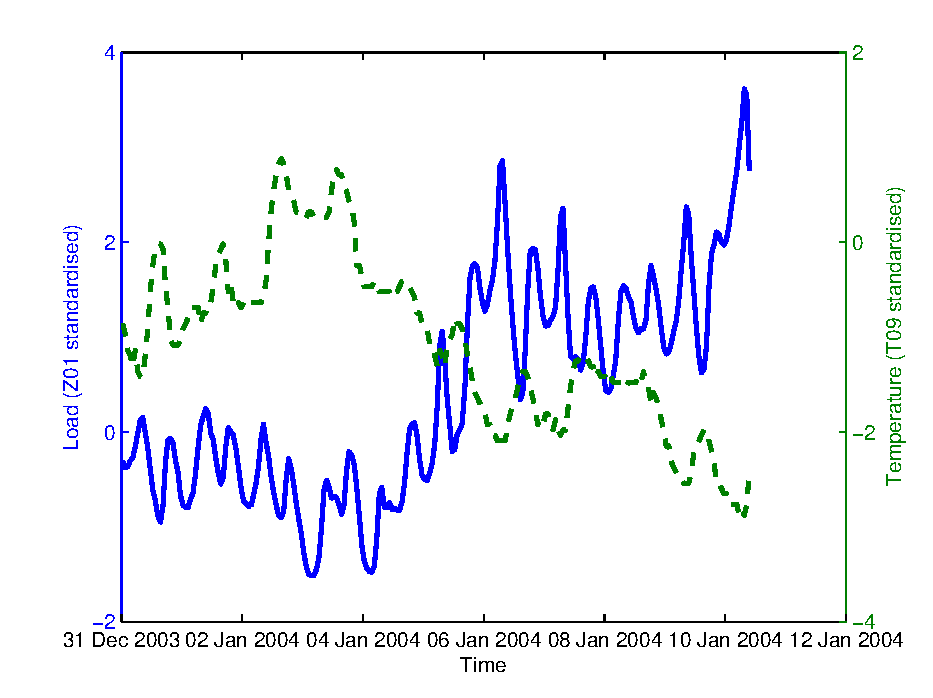
\includegraphics[width=12cm]{include/gef_load_z01_t09_250.pdf}
    };
  \end{scope}
\end{tikzpicture}

  \end{center}
  \caption{Raw data at load zone 1 (after removing mean and scaling to have unit standard deviation) (blue) and raw data at temperature station 9 (after removing mean and scaling to have unit standard deviation) (green).}
  \label{fig:load_temp}
\end{figure}

Figure~\ref{fig:load_temp} plots a subset of the data for loads at zone 1 and temperature station 9.
We can see that that the load has a smoothly varying trend with roughly periodic daily deviations from this trend.
The load also appears to be negatively correlated with temperature in this region of data.

Based on these observations, I used gradient boosting machines to model loads as a function of time of day, temperatures (all stations) and smoothed temperatures.
All zones were modelled independently.

\subsection{Methodology}

A standard `black-box' technique for learning an unknown (regression) function is that of using gradient boosting machines (GBM) \citep[e.g. chapter 10 of][]{Hastie2009}.
For each zone I used all of the data to train a GBM and then used that to predict all outputs \ie I learnt a global function for each zone.

I used a standard R implementation of GBM using most of the default settings\footnotemark.
After some brief experimentation with parameter values I used a shrinkage factor of 0.01, 10000 trees and an interaction depth of 3.
I experimented with other parameter values, using the public test score as a guide, but nothing I tried improved on my initial guess and therefore I did not expend much effort trying to optimise parameter values.

\footnotetext{\url{http://cran.r-project.org/web/packages/gbm/index.html}}

\subsection{Replication of results}

The scripts and data used can be found in the folder \texttt{gbm}.
The load data was reshaped into a (time) $\times$ (load zone) array using the spreadsheet \texttt{load.xlsx} in the folder \texttt{load}.
This was then concatenated with the temperature predictions and smoothed temperature predictions and saved in \texttt{Z\_t\_T\_no\_year.csv}.
The R script \texttt{basic\_gb.R} then performs the method described above to produce predictions which are saved in \texttt{basic\_gb\_Z\_t\_T\_no\_year\_pred.csv}.

\subsection{Discussion}

The time series for zone 10 had a very large discontinuity.
GBM was used as a global prediction method which means it will have produced very bad predictions for zone 10.
I later fixed this by modelling the loads either side of the discontinuity separately.
Perversely this resulted in a worse public test score.
However, this change resulted in a much improved private test score; in hindsight I should have opted for the more reasonable model!

\section{Gaussian processes}

\subsection{Initial analysis and remarks}

The observations made about the load data in section~\ref{sec:gbm_init_anal} (\ie smooth trends, near periodic variations, dependence on temperature) can be modelled using Gaussian process regression.
Specifying the kernel function of a Gaussian process allows us to encode these structural assumptions into a Bayesian nonparametric analysis that can learn the details of the regression function from the data (see the appendix for a brief introduction to the effect of choosing different kernels).

\subsection{Methodology}

Three different kernel functions were used; one for backcasting, one for forecasting and one for backcasting zone 9.
The three kernels used were as follows
\begin{eqnarray}
S_t + S_S + S_t \times S_T \times P_t \label{eqn:kernel1}\\
S_t + S_t + P_t \label{eqn:kernel2}\\
S_t + S_S + S_T \times P_t\label{eqn:kernel3}
\end{eqnarray}
where $S$ refers to a squared exponential kernel, $P$ is a periodic kernel and the subscripts indicate which dimension the kernel acts upon; (t)ime, (T)emperature or (S)moothed temperature.
For backcasting, the model was applied to the 1000 surrounding data points; for forecasting the last 500 data points were used.
Only one temperature station was used in this method; for each back/forecasting region the marginal likelihood of the data was computed for each temperature station.
Bayesian model averaging \citep[e.g.][]{Hoeting1999} was then used to combine the predictions (in practice, this was almost numerically equivalent to selecting the model/temperature station with the highest marginal likelihood).

Kernel~\eqref{eqn:kernel1} encodes the assumptions that loads can be explained as a smoothly varying trend and an approximately periodic component.
The smooth trend is the sum of a smooth function of smoothed temperature and a smooth function of time (to explain any deviations from the trend implied by temperature).
The periodic component can vary through time and by being multiplied by $S_t$ and $S_T$ the shape of the periodicity will be more similar to recent times and points in time with similar temperatures.
This kernel was used for backcasting all zones apart from zone 9.
An example of this kernel in action is shown in figure~\ref{fig:load_pred}.
The top plot shows the load data (black) and the prediction (red).
Below is the temperature time series which resulted in the model with the highest marginal likelihood.
Comparing the two plots we can see that the deviations of the prediction from the trend through time correspond to fluctuations in the temperature time series.

\begin{figure}[ht]
  \begin{center}
    \begin{tikzpicture}
  \begin{scope}[xshift=0cm]
    \node [mybox] (box){
      \includegraphics[width=0.5\textwidth]{../include/load_pred.pdf}
    };
  \end{scope}
  \begin{scope}[xshift=0.5\textwidth]
    \node [mybox] (box){
      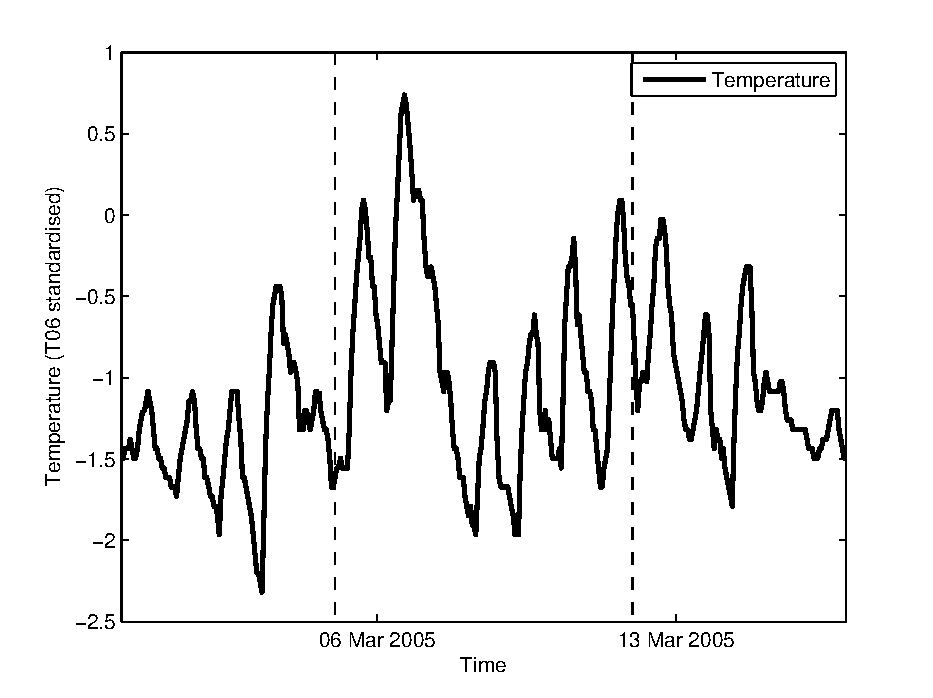
\includegraphics[width=0.5\textwidth]{../include/best_temp.pdf}
    };
  \end{scope}
\end{tikzpicture}

  \end{center}
  \caption{Top: Raw data (after scaling and translation) (black) and Gaussian process predictions (red) for zone 1. Bottom: Corresponding temperature time series used for prediction.}
  \label{fig:load_pred}
\end{figure}

Kernel~\eqref{eqn:kernel2} encodes the assumption that loads can be explained as the sum of two smooth functions with different length scales and an exactly periodic smooth function.
This simpler kernel was used for forecasting since it gave more stable extrapolations of the data.

Kernel~\eqref{eqn:kernel3} is a simpler version of kernel~\eqref{eqn:kernel1} used for backcasting zone 9.
The periodic component is now only similar to other times with similar temperatures.
This prevented the predictions from being so greatly affected by the large isolated load fluctuations present in zone 9.

The forms and parameters of the kernel functions (see the accompanying code for all of the values) were chosen by trial and error (observing which kernels gave reasonable looking predictions and computing public test scores).

\subsection{Replication of results}

The spreadsheet and scripts used can be found in the folder \texttt{gp}.
The load data was reshaped into a (time) $\times$ (load zone) array using the spreadsheet \texttt{load.xlsx} in the folder \texttt{load} and then saved in \texttt{Z\_t\_with\_zeros.csv} which encodes missing values as zeros.
The outputs of the temperature prediction \texttt{GP\_pred\_temp\_008.csv} and \texttt{smooth\_temp\_GP\_08.mat} are used directly.

The MATLAB script \texttt{gp\_elec\_predict\_load\_v04.m} performs the methodology described above, saving the predictions to \texttt{gp\_elec\_GP\_pred\_covElec07.csv}.

\subsection{Discussion}

Selecting the form and parameters of the kernels by hand requires a moderate amount of familiarity with Gaussian processes.
Automatic selection of kernel functions is an active area of research \citep[e.g.][]{DBLP:journals/corr/abs-0909-0844, diosan2007evolving, duvenaud2011additive11} to cite but a few different approaches.
It is likely that better performance could have been achieved by a larger and more principled search over kernel functions.

\section{Selecting the final ensemble}

\subsection{Remarks}

The final prediction was formed as the ensemble (weighted average) of predictions from three separate methods; gradient boosting machines, Gaussian process regression and the benchmark solution provided by the competition organisers (a linear model).
Ensembling is a very powerful technique for combining predictions from separate models.
If two predictions (viewed as random quantities) are statistically uncorrelated then their average will have lower variance than either one separately.

In practice, different algorithms are correlated and ensembling highly correlated predictions will rarely lead to improved performance.
In particular, I also tried the random forest algorithm but the predictions were too correlated with gradient boosting machines (they are both based on an ensemble of decision trees) to be a useful component in an ensemble.

\subsection{Methodology}

The ensemble weights were chosen by hand, using the public test score as the metric to be optimised.
The public test scores did not vary considerably once sensible parameters had been found so more advanced techniques were not used to optimise the ensemble weights.

\subsection{Replication of results}

The spreadsheets used to manipulate model output can be found in the folder \texttt{ensemble}.
The spreadsheet \texttt{sub\_creator.xlsx} was used to convert (time) $\times$ (load zone) arrays of model output into the required format for submission.
The output of this spreadsheet was then copied in \texttt{ensemble\_creator.xlsx} which performs the necessary averaging to produce ensembles of the predictions.

\subsection{Discussion}

This method could have been been slightly improved by programmatically selecting the ensemble weights, optimising some form of validation metric.
One could also have tried to optimise the public test score directly.
Since only 2 submissions could be tested per day, one would want to use an optimisation technique that made very efficient use of data \citep[e.g.][]{Osborne2009}.

Larger improvements could likely be achieved by considering a larger number of base predictions.
It is likely that the algorithms used by other competitors in GEFCom2012 would provide useful additions to the ensemble of predictions.

\section{Conclusion}

In this competition I applied general purpose machine learning algorithms and made few adjustments for the specific domain the data arose from.
Despite this, the resulting predictions were highly competitive.
It is hoped that this report shows that simple techniques can be very effective for predictive modelling and can inspire practical techniques for load forecasting.

% use section* for acknowledgement
\section*{Acknowledgment}

I would like to thank Alex Davies for his guidance into the ways of data mining and David Duvenaud for advice on the practicalities of using Gaussian processes.

\appendix

\section{A very brief introduction to Gaussian processes}

For a much richer introduction, see \cite{Rasmussen2006}.
A Gaussian process, $(f_x)_{x \in X}$ is a set of random variables such that any finite collection has a jointly Gaussian distribution.
A Gaussian process can be completely specified by a mean function $m(x)$ and kernel function $\kappa (x, x')$ such that
\begin{eqnarray}
\text{Expectation}(f_x) & = & m(x) \\
\text{Covariance}(f_x, f_{x'}) & = & \kappa (x, x').
\end{eqnarray}

Gaussian processes can be used to specify a prior distribution on functions and then be used in a Bayesian analysis.
They are nonparametric and can learn any function given sufficient data.

\begin{figure}[ht]
  \begin{center}
    \begin{tikzpicture}
  \begin{scope}[xshift=0cm]
    \node [mybox] (box){
      %\includegraphics[width=9.0cm]{include/load_pred.pdf}
      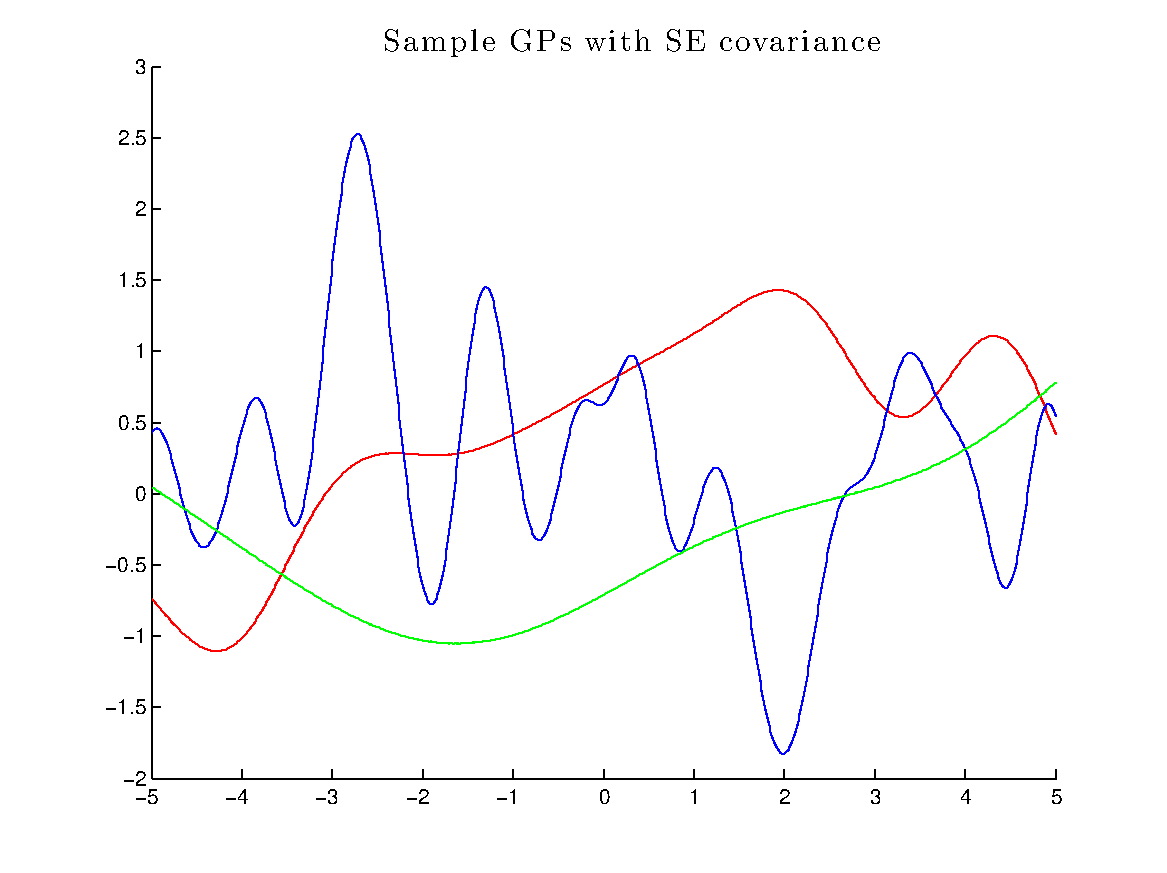
\includegraphics[width=7.0cm]{include/Part_d_1.pdf}
    };
  \end{scope}
  \begin{scope}[xshift=7.0cm]
    \node [mybox] (box){
      %\includegraphics[width=9.0cm]{include/load_pred.pdf}
      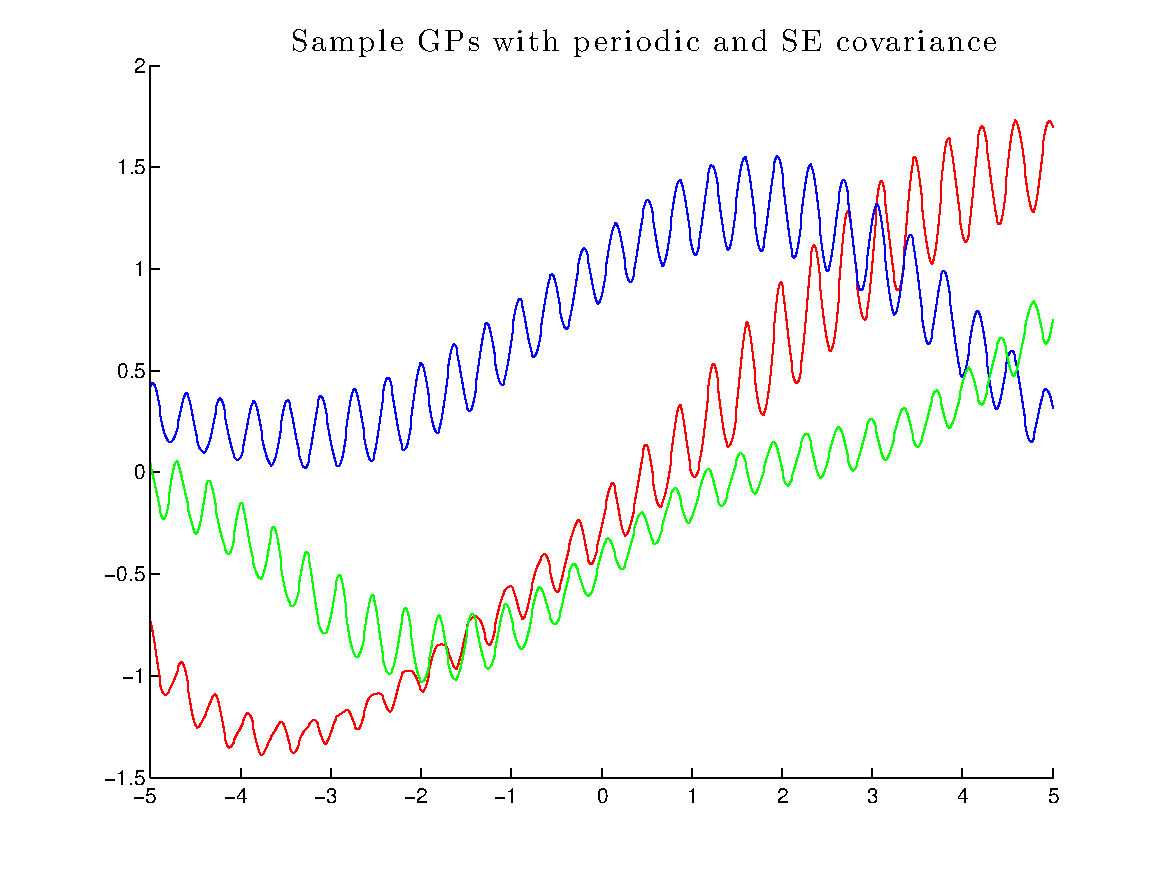
\includegraphics[width=7.0cm]{include/Part_d_2.pdf}
    };
  \end{scope}
\end{tikzpicture}

  \end{center}
  \caption{Top: Draws form a Gaussian process with squared exponential kernel with differing length scales. Bottom: Draws using a squared exponential and periodic product kernel.}
  \label{fig:gp_samples}
\end{figure}

The kernel function encodes the structure of a Gaussian process.
The top plot in figure~\ref{fig:gp_samples} shows samples (random draws) from a Gaussian process distribution using squared exponential kernels; this function encodes an assumption of smoothness.
Intuitively, these plots show the types of functions that will most easily/quickly be learned using Gaussian process regression.
One parameter of a squared exponential kernel is a length scale which controls how quickly the value of the Gaussian process varies.
The blue line in the top plot has a short length scale which results in quick variations of the function.
The green line has a long length scale and consequently the Gaussian process is visually much smoother.

The bottom plot in figure~\ref{fig:gp_samples} shows samples from a Gaussian process with a more complicated kernel function.
The kernel function is the product of a squared exponential kernel and a periodic kernel.
This encodes the assumption that the Gaussian process is roughly periodic, and that the shape of the periodicity changes smoothly.

By constructing more advanced kernel functions one can specify more complex structures as desired.
Kernel functions depend on parameters and they are typically chosen by maximising the marginal likelihood of training data given the parameter choices (all gradients can be computed analytically).
One can also perform a fully Bayesian analysis by integrating over parameter values; this typically requires approximate inference techniques.

%% References with bibTeX database:

\bibliographystyle{elsarticle-harv}
\bibliography{library}

\end{document}
